%\section{Kalman Filter Overview} \label{KF_SECT}
\section{Kalman Filters} \label{KF_SECT}
\subsection{A General Overview of Kalman Filtering}
Kalman Filters (KF) fall under the umbrella of Machine Learning models, however are additionally an example of a mechanistic model, meaning that it allows us to gain an understanding of the individual, inner workings of complex systems. Moreover, unlike MCMC's, which are used on already fully obtained data sets, Kalman Filters can be adjusted as new data is brought in \cite{ChowFerrer}. This makes Kalman Filters unique in that they can operate in real time as well. Rather than making predictions using an entire dataset at once, KFs improve and evolve as more datapoints are assessed. To use a KF, the system must be in a discretized state space form \cite{SimonHaykinText}. To do this, one must identify two sets of variables: latent states and observables.\\

Latent states are the set of variables that one is interested in estimating, which can include values such as a population count or model parameters. On the other hand, observables are a set of data which has been measured from the system and is the only piece of information known about the system at a particular time point \cite{ChowFerrer}. \\

Additionally, Kalman Filters are helpful due to their ability to quantify the noise associated with a system. This is achieved through both process and measurement noise. Process noise describes outside forces and situations which, as a result of their actions, affect states in the model. Measurement noise, on the other hand, accounts for the fact that tools to gather observable data may be inherently flawed, and thus some level of noise is associated with the values they produce \cite{ChowFerrer}. In order to gather a holistic, high level understanding of Kalman Filters, consider the example of a car driving down a street.\\

Assume that one observes a car at time $t$ traveling at a velocity of $Y$ m/s at a position of $X$ m from an observed starting point, as seen in Figure \ref{fig:Car_Example}. In order to estimate what the car's velocity will be at time $t+1$, one may choose to utilize a Kalman Filter. Assuming that the position at time $t+1$ can be measured to be $Z$ m with a device such as a ruler, this position thus is the observable, while the velocity is a latent state. However, since the tool is flawed, measurement noise is added in as well. If we assume that while this is occurring, a force of $W$ Newtons pushes from above the car, this would now become a source of process noise. Having all of this information, one is now capable of applying a KF to estimate the velocity of the car at time $t+1$.\\

\begin{figure}[H]
    \centering
    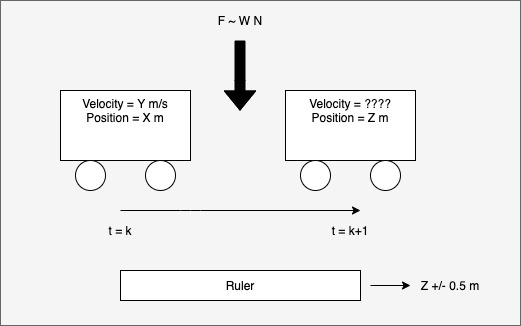
\includegraphics[width=15cm]{Kalman_Filter_Images/Cart_Example.jpg}
    \caption{A visualization of utilizing a Kalman Filter to estimate the velocity of a car. Here, the latent state is the velocity while the observable is the distance.}
    \label{fig:Car_Example}
\end{figure}

As stated earlier, Kalman Filters operate in discrete time, state space models, meaning that input and output variables are being related to one another through a system of ODEs at known time points. Thus, we must have knowledge about the system to the extent that we know the structure of the ODEs, although as we'll see, there are formats of the Kalman Filter in which it is not necessary to know the parameter values. Having both an understanding of the ODEs and the observable data, we can now introduce the the projection and update steps, the two of which drive the KF algorithm and are visualized in Figure \ref{fig:UKF_TwoSteps}. 
%{The simplest use of Kalman Filters is for state estimation, which we will describe in the following sections. Although our eventual goal is to implement parameter estimation, since parameter estimation is based on the foundation of state estimation, it is easier to understand if you first have a general understanding of state estimation. As a result of this, we will introduce  parameter estimation later on.%} 

\begin{figure}[H]
    \centering
    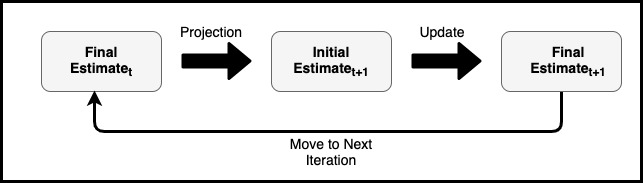
\includegraphics[width=15cm]{Kalman_Filter_Images/Simple_UKF_Flow.jpg}
    \caption{The two steps of the Kalman Filter algorithm. First, we use knowledge of the system to create an initial prediction, following which observable data is produced to produce final estimates.}
    \label{fig:UKF_TwoSteps}
\end{figure}

\textbf{Projection Step}: The first step of the KF relies only on knowledge of the system. Having an estimate of latent states at time $t$, we use our knowledge of the system to predict the states at time $t + 1$, known as the prior estimate \cite{SimonHaykinText} \cite{GoveHollingerDual}.\\

\textbf{Update Step}: Having a prior estimate, we can now bring in the observable data. By seeing how the prediction we made in the Projection Step compares to the observable data, we now update our predictions and states \cite{GoveHollingerDual}. This is now our posterior estimate \cite{SimonHaykinText}, and becomes the set of states that are projected forward to produce the prior estimate for time $t+2$. We continue this loop as long as new data is coming in, continously improving results as more data arrives. \\
\\


\subsection{Introduction to Kalman Filters}
    Please note that all notation and equations in this section and section \ref{section:UKF_Theory} are adapted from \cite{VanMereChapter} and \cite{SimonHaykinText}, two sources we have found very helpful in guiding our understanding of Kalman Filters.
    \subsubsection{Different Types of Kalman Filters}
    Multiple formulations of Kalman Filters exist for different types of systems. When a system is linear, one may use the standard Linear Kalman Filter. However, once the system becomes nonlinear this is no longer feasible. If the nonlinear system may be accurately linearized with first order Taylor approximations, the Extended Kalman Filter (EKF) may be used. The theory for the EKF is based around the first order Taylor approximation. However, if the nonlinear system  is not easily linearized, it is recommended to use the Unscented Kalman Filter (UKF) \cite{VanMereChapter}. Due to the inability of complex ODE systems to be accurately approximated with first order Taylor approximations, we will focus on the Unscented Kalman Filter here.
    
    \textbf{A Note on Parameter Estimation} The general UKT, which we will describe in the following sections is built for state estimation purposes. However, the UKF can also be used for parameter estimation, which is the context in which it will be used when describing its implementation. Specifically, we will be using the UKF to estimate states and parameters at the same time via the Joint and Dual methods, described in section \ref{section:Parameter_Estimation}.
    
    
    
    \subsubsection{Process and Measurement Equations}
    The Unscented Kalman Filter is used to estimate the states of a nonlinear system. The system, set up as a state space model, is described by the process and measurement equations \cite{SimonHaykinText}. The process equation, describing the transition of the latent states from time $k$ to time $k+1$ is formulated as
    \begin{equation}
    x_{k+1} = F_{k+1,k}(x_k) + q_k, 
    \end{equation}
    where $x_{k}$ is the vector of states at time $k$, $x_{k+1}$ is the vector of states at time $k+1$, $F$ is the non-linear transition function that takes the state from time $k$ to time $k+1$, and $q_k$ is the process noise \cite{SimonHaykinText}. $F$ and $q_k$ are assumed to be known quantities. The latent states are the variables that we are trying to estimate. The Measurement equation, describing the relationship between observed data points and the unknown states, is 
    \begin{equation}
    y_k = H_k(x_k) + r_k,  
    \end{equation}
    where $y_k$ is the vector of the observables, $H$ is a (possibly) nonlinear function that relates the states to the observables, and $r_k$ represents the measurement noise \cite{SimonHaykinText}. Often times, only some sort of algebraic combination of states can be observed. For example, if the latent state is simply $x$, we may only be able to observe $3x^2$. Thus, the purpose of $H$ is to relate the actual observed value, $3x^2$ to the latent state $x$.\\
    \\
    $H$ and $r_k$ are assumed to be known in the Measurement equation. 
    \subsubsection{Set up of the Noise}
    The above system of equations relies on both process and measurement noise. The vector $q_k$, which follows the same dimensions as the state vector in order to apply one noise value to each state, describes the process noise and is multivariate Gaussian with mean 0 and covariance described by 
    \begin{equation}
    E[q_{n}q_{k}^T] = \Bigg\{\begin{tabular}{l}
    $Q_k$\ for\ n = k  \\
    0   for \ $n \neq k$
    \end{tabular}.
    \end{equation}
    
    Similarly, $r_k$ describes the measurement noise and is Gaussian with mean 0 and covariance described by 
    \begin{equation}
    E[r_{n}r_{k}^T] = \Bigg\{\begin{tabular}{l}
    $R_k$\ for\ n = k  \\
    0   for \ $n \neq k$
    \end{tabular}. 
    \end{equation}
    
    
    Both of these covariance matrices will play a role in the UKF calculations. Furthermore, it is important to note that our system assumes white, additive noise. If we have a system where the noise is not additive, the Kalman Filter equations must be altered, which can be seen in \cite{VanMereChapter}. 
    
    \subsubsection{Unscented Transformation}
    Developed in response to the shortcomings of Kalman Filters on nonlinear systems, The Unscented Kalman Filter is formulated around the Unscented Transformtation (UT) \cite{JulierPaper}. The UT is used to understand the distribution of a random variable after a nonlinear transformation has been applied to it \cite{JulierPaper}. 
    \\
    To understand the distribution of a random variable post a nonlinear transformation, the UT creates a set of \textbf{sigma vectors} meant to capture points in the distribution in an ideal, deterministic fashion \cite{JulierPaper} \cite{VanMereChapter}. Consider random variable $v$, i.e.
    
    \begin{equation}
    v = \begin{bmatrix} v_1\\ v_2\\v_3\\.\\.\\.\\v_L\end{bmatrix},
    \end{equation}
    
    with dimensions $L$ x $1$. Additionally, consider a different random variable $z$ that is some function of $v$ such that $z = f(v)$. Also assume that the distribution of $v$ has mean $\bar{v}$ and covariance $P_v$. To understand the distribution of the nonlinear transformation y, we create an $L$ x $2L+1$ matrix $\chi$ of 2$L$ + 1 sigma vectors as follows:
    \begin{equation} \label{eq:UT_1}
    \chi_0 = \bar{v}
    \end{equation}
    \begin{equation} \label{eq:UT_2}
    \chi_i = \bar{v} + (\sqrt{(L + \lambda)P_v})_i \ i = 1 ... L
    \end{equation}
    \begin{equation} \label{eq:UT_3}
    \chi_i = \bar{v} - (\sqrt{(L + \lambda)P_v})_{i - L} \ i = L + 1 \  ...  \ 2L + 1.
    \end{equation}
    The number 2$L$+1 gives us one vector at the mean, or expectation, of the random variable and $L$ vectors above and below the mean. As stated above, $L$ is the dimension of $v$ which means it is number of states in our system. The subscript $i$ refers to the $i$th columns in the matrix square root of the term $(\sqrt{(L + \lambda)P_v})$.\\

    Here, $\lambda$ is a final scaling parameter defined as $\alpha^2(L + k) - L$, where $\alpha$ is a scaling parameter that represents the spread of vectors around $\bar{v}$. $k$ is a secondary scaling parameter, set to either 0 or $3-L$, whereas $\alpha$ takes on a value between 10e-4 and 1 \cite{VanMereChapter}. It is crucial to note that this is a form of \textbf{deterministic} scaling. In many sampling schemes, sampling is done \textbf{randomly} from a distribution. However, here our goal is to choose points in equal intervals and in equal quantities of either side of the mean, $\bar{v}$. The purpose of this is so that we may be certain that sigma points accurately capture the spread of a distribution. With random sampling, if only choosing a small amount of points, we can make no guarantees about the distribution of these points. Thus, exact equations are given for how the sigma vectors should be chosen. \\
    \\
    Once $\chi$ has been calculated, the sigma vectors are then sent through the nonlinear function $f$ to create vectors $Z_i$. This is done as follows:
    \begin{equation}
    Z_i = f(\chi_i) \ \ i = 0,...,2L.
    \end{equation}
    
    Now, by weighting these output vectors $Z_i$ in a deterministic fashion, we can calculate a mean and covariance in order to understand our new distribution \cite{VanMereChapter}. In order to do this, we create the following weights, where $W^{(m)}$ are weights corresponding to calculating the mean and $W^{(c)}$ is used to calculate our covariance:
    \begin{equation} \label{eq:Weights_1}
    W_0^{(m)} = \lambda/(L + \lambda),
    \end{equation}
    \begin{equation} \label{eq:Weights_2}
    W_0^{(c)} = \lambda/(L + \lambda) + (1 - \alpha^2 + \beta),
    \end{equation}
    \begin{equation} \label{eq:Weights_3}
    W_i^{(m)} = W_i^{(c)} = 1/(2(L + \lambda)) \ i = 1 ... 2L.
    \end{equation}
    Here, $\beta$ holds prior knowledge about the distribution (for Gaussian $\beta = 2$ is used) \cite{VanMereChapter}. We can see that the sigma point that represents the mean is given more weight than the others. Now the mean and covariance can be calculated:
    \begin{equation}
     \bar{z} \approx \sum_{i = 0}^{2L} W_i^{(m)} Z_i,
    \end{equation}
    \begin{equation}
    P_z \approx \sum_{i = 0}^{2L} W_i^{(c)}(Z_i - \bar{z})(Z_i - \bar{z})^T.    
    \end{equation}
    Understanding this mean and covariance will be useful in creating our prior estimates in the UKF method.
    \\
    
    For a visual representation of the importance of the UT, see Figure \ref{fig:UT_Diagram_Custom}.
    \begin{figure} [H]
    \centering
    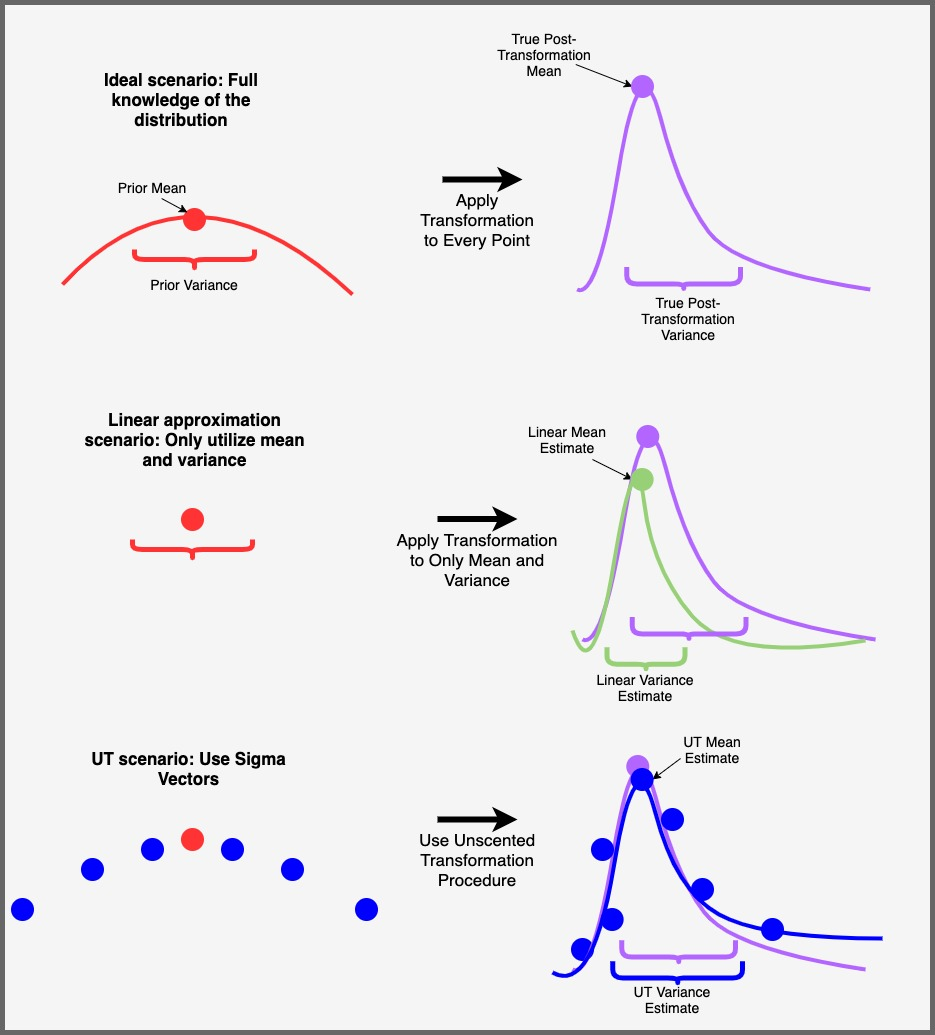
\includegraphics[scale = .5]{Kalman_Filter_Images/Unscented_Transformation_Diagram.jpg}
    \caption{A comparison of 3 techniques to understand the distribution of a transformation of a random variable. At the top, we see an ideal schema where we have full knowledge of a distribution and can transform every point to understand the true mean and covariance of the RV post-transformation, as seen in purple. In the second row, we linearize the transformation and only transform the mean and variance. However, this does not produce a good approximation, which is shown in green. Lastly, we use the UT to deterministically choose sigma vectors that are transformed and then weighted to more accurately capture the new mean and variance, as shown in blue.}
    \label{fig:UT_Diagram_Custom}
    \end{figure}
    
    Figure \ref{fig:UT_Diagram_Custom} visualizes the importance of the Unscented Transformation. In an ideal scenario, one has full knowledge of a RV's distribution and can thus apply the transformation to every single possible point to understand the new mean and variance. However, we often need ways to approximate the nonlinear transformation. One naive solution is to linearize the transformation and only transform the mean and variance, however this results in not as accurate of a fit \cite{VanMereChapter}. The solution to this issue is the Unscented Transformation. By deterministaclly choosing the blue sigma vectors, applying the transformation, and then weighting these transformed vectors, we are able to much more closely capture the actual mean and variance of the RV post-transformation. As a result, sigma vectors play a key role in the inner-workings of the Unscented Kalman Filter.\\
    
    Having a theoretical understanding of the UT, we can now discuss the specifics of the UKF algorithm.
    
    \subsection{Theory of the Unscented Kalman Filter} \label{section:UKF_Theory}
    
    \subsubsection{Notation}
    Before delving deeper into the process of using a Kalman Filter, it is important to establish the notation that will be used throughout. This notation is adapted from \cite{SimonHaykinText} and \cite{VanMereChapter}.
    \paragraph{States Notation}
    For our states, we first have $\hat{x}_0$ for our initial posterior estimate. Next, we notate our prior estimate as $\hat{x}_k^-$ and our posterior estimate, following the Update Step, as $\hat{x}_k$. Then, we have analogous notation for the states covariance. Namely, we start with $P_0$, have a prior estimate of $P_k^-$, and then a posterior covariance of $P_k$.
    \paragraph{Observables Notation}
    We must define similar notation for our observables. Here, we have a prior estimate $\hat{y}_k^-$, but instead of a posterior estimates, we have the \emph{actual} observable value $y_k$. Using these two values, we also define the error, or \emph{innovation}, as:
    \begin{equation}
    \tilde{y}_k = y_k - \hat{y}_k^-.    
    \end{equation}
    Then, we once again have a covariance matrix, but this time for the innovation, $P_{\tilde{y}_k}$. This is the basis of the notation, however more will be introduced as necessary in the following sections, and a full guide can be found in Table \ref{table:KF_Notation}.
    
    \subsubsection{Initialization}
    The initial states vector $x_0$ and the initial covariance matrix between the states, $P_0$, are needed to initialize the UKF. To create these initial guesses some prior knowledge of the states and their plausible ranges is necessary. Assuming this information is available, one may initialize with:
    \begin{equation}
    \hat{x}_0 = E[x_0],
    \end{equation}
    and initial covariance matrix:
    \begin{equation}
    P_0 = E[(x_0 - \hat{x}_0)(x_0 - \hat{x}_0)^T].
    \end{equation}
    \cite{VanMereChapter}
    When working with real data, one is not likely to have a full understanding of the states' distribution. Thus, a first guess will suffice and may be tuned throughout working with the UKF, as will be discussed in section \ref{KF_General_Implementation}.  
    \subsubsection{Projection Step}
    Now, we proceed to do the projection portion of the algorithm. Having chosen a set of sigma points via equations \ref{eq:Weights_1}, \ref{eq:Weights_2}, and \ref{eq:Weights_3} , we now project them in time by applying the transition matrix to each point in the vector $\chi_{k-1}$:
    \begin{equation}
    \chi_{k|k-1} = F(\chi_{k-1}).
    \end{equation}
    It is important to note that here $\hat{x}_{k-1}$ plays the role of $\bar{v}$ in equations \ref{eq:UT_1}, \ref{eq:UT_2}, and \ref{eq:UT_3}.
    Next we calculate a prior prediction of the state $\hat{x}_k^-$ with:
    \begin{equation}
    \hat{x}_k^- = \sum_{i = 0}^{2L} W_i^{(m)} \chi_{i, k|k-1}.
    \end{equation}
    Similarly we can calculate a prior covariance $P_k^-$ by using our weights as well as the process noise:
    \begin{equation}
    P_k^- = \sum_{i = 0}^{2L} W_i^{(c)} [\chi_{i, k|k-1} - \hat{x}_k^-][\chi_{i, k|k-1} - \hat{x}_k^-]^T + Q.
    \end{equation}
    We can see that the calculation of $\hat{x}_k^-$ and $P_k^-$ are both \emph{applications of the Unscented Transformation} as we created, transformed, and weighted sigma vectors. Next, we apply the UT transformation to understand our observables with:
    \begin{equation}
    Y_{k|k-1} = H[\chi_{k|k-1}].
    \end{equation}
    This allows us to know calculate a prior estimate of the observables $y_k^-$ by utilizing:
    \begin{equation}
    \hat{y}_k^- = \sum_{i=0}^{2L} W_i^{(m)} Y_{i,k|k-1}.
    \end{equation}
     Once again, we have made use of the \emph{UT transformation} here by passing our sigma vectors through $H$ this time, as opposed to $F$ as before.
    \subsubsection{Update Step}
    Having created prior estimates for both states and observables, we now proceed to the update step where the observed data is brought in \cite{VanMereChapter}. \\
    
    We begin by calculating the covariance matrix $P_{\tilde{y}_k, \tilde{y}_k}$, which is the covariance matrix for the error between the projected and actual values of the observables. \\
    
    Moreover, this calculation takes into account the measurement noise through $R$:
    \begin{equation}
    P_{\tilde{y}_k, \tilde{y}_k} = \sum_{i=0}^{2L} W_i^{(c)} [Y_{i,k|k-1} - \hat{y}_k^-][Y_{i,k|k-1} - \hat{y}_k^-]^T + R. 
    \end{equation}
    Next we need a covariance between our states and observables, which is calculated by:
    \begin{equation}
    P_{{x}_k,{y}_k} = \sum_{i=0}^{2L} W_i^{(c)} [\chi_{i,k|k-1} - \hat{x}_k^-][Y_{i,k|k-1} - \hat{y}_k^-]^T.
    \end{equation}
    At this point, we have sufficient information to calculate the \textbf{Kalman Gain}, a crucial term in the UKF algorithm. The Kalman Gain is used to weight the error between the predicted value and the observed value of $x_k$ in order to update the filter's prior predictions. A larger Kalman Gain will give more weight to the error, resulting in a larger correction and a smaller Kalman Gain will give less weight to the error, resulting in a smaller correction. The Kalman Gain is also used to adjust the covariance matrix $P_k$ and is calculated through \cite{VanMereChapter}:
    \begin{equation}
    K_k = P_{x_k, y_k} P_{\tilde{y}_k, \tilde{y}_k}^{-1}. 
    \end{equation}
    Calculation of the Kalman Gain allows us to calculate our posterior estimates of both the states, $\hat{x}_k$, and covariance, $P_k$ \cite{VanMereChapter}. For the states the following equation is used
    \begin{equation}
    \hat{x}_k = \hat{x}_k^- + K_k(y_k - \hat{y}_k^-). 
    \end{equation}
    And for the covariance we use:
    \begin{equation} \label{eq:27ukf}
    P_k = P_k^-  - K_k P_{\tilde{y}_k, \tilde{y}_k} K_k^T.
    \end{equation}
    We can see that both equations function by adjusting our prior prediction through use of the Kalman Gain.\\
    \\
    After having gone through the update step, the next data point would be brought in and we would return to the Projection Step once more.
    \subsubsection{Summary}
    A flow chart depicting one iteration of the entire UKF process is found in figure \ref{fig:UKF_Theory_FlowChart}. To summarize, our goal is to begin with a set of sigma points chosen in a deterministic fashion and arrive at the posterior estimates for the states and covariance. This is done in two main sections, the Projection Step, whose quantities are shaded in red, and the Update Step, displayed in blue.
    
    \begin{figure} [H]
    \centering
    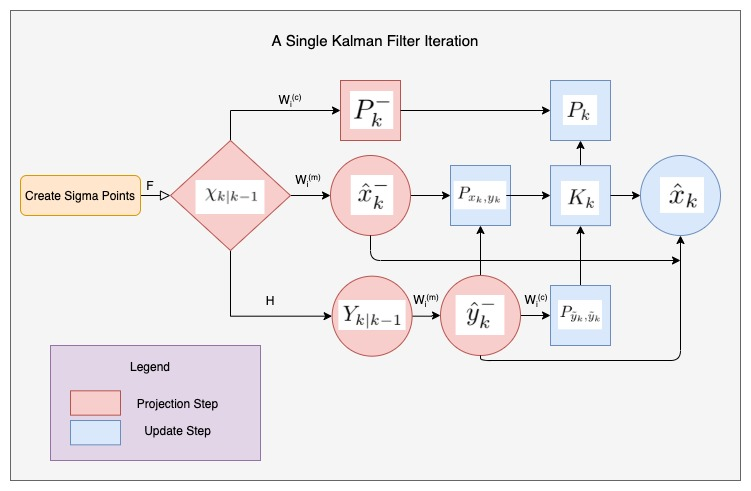
\includegraphics[scale = 0.6]{Kalman_Filter_Images/UKFFlowDiagram.jpg}
    \caption{A flow chart depicting one iteration of the UKF process. The sigma points are shaded in yellow, the intermediate steps in red, the Kalman gain in green, and the posterior estimates in blue.}
    \label{fig:UKF_Theory_FlowChart}
    \end{figure}
    
    \subsubsection{Stability and Divergence Issues}
    When utilizing the UKF, it is important to consider the issue of positive definitiness of the covariance matrix $P_k$. If this matrix becomes non-positive definite, the filter can experience severe divergence issues due to invalid covariance matrices, which can occur as a result of the update made in equation \ref{eq:27ukf}. This then can lead the filter to diverge \cite{SimonHaykinText}. \\
    
    The solution to the issue lies in using the \textbf{Cholesky factorization} \cite{SimonHaykinText}.
    \\
    
    At every iteration of the Kalman Filter, one must perform the following step:
    \begin{equation}
    P_k = {P_k}^{1/2} {P_k}^{T/2},
    \end{equation}
    where ${P_k}^{1/2}$ is the \textbf{Cholesky factor} and is in lower-triangular form, and ${P_k}^{T/2}$ is the Cholesky factor's transpose \cite{SimonHaykinText}. Here, $P_k$ is now the product of a square matrix and its transpose, which is \textbf{guaranteed to be positive definite}. In order to find the Cholesky factor, a function such as Matlab's \emph{chol} (https://www.mathworks.com/help/matlab/ref/chol.html) can be used. By using this approach, one will have a better chance of maintaining the stability of the Kalman Filter across iterations. \\

    
\begin{tcolorbox} [breakable, enhanced]

\textbf{\underline{The Unscented Kalman Filter Algorithm With Additive Noise}} 
\begin{enumerate}
    \item Initialize $\hat{x}_0 = E[x_0]$ or with best guess.
    \item Initialize $P_0 = E[(x_0 - \hat{x}_0)(x_0 - \hat{x}_0)^T]$ or with best guess.
    \item For each incoming data point perform the following:
    \begin{enumerate}
        \item Projection Step
        \begin{enumerate}
            \item Create Sigma Points 
            \begin{itemize}
                \item  $\chi_0 = \bar{x}$
                \item $ \chi_i = \bar{x} + (\sqrt{(L + \lambda)P_x})_i \ i = 1 ... L $
                \item $ \chi_i = \bar{x} - (\sqrt{(L + \lambda)P_x})_{i - L} \ i = L + 1 \  ...  \ 2L + 1 $
            \end{itemize}
            \item Project Sigma Points forward with
            $$\chi_{k|k-1} = F(\chi_{k-1})$$
            \item Calculate prior state estimate
            $$ \hat{x}_k^- = \sum_{i = 0}^{2L} W_i^{(m)} \chi_{i, k|k-1}$$
            \item Calculate prior covariance estimate 
            $$ P_k^- = \sum_{i = 0}^{2L} W_i^{(c)} [\chi_{i, k|k-1} - \hat{x}_k^-][\chi_{i, k|k-1} - \hat{x}_k^-]^T + Q$$
            \item Project observables forward with 
            $$Y_{k|k-1} = H[\chi_{k|k-1}]$$
            \item Calculate prior observable estimate 
            $$\hat{y}_k^- = \sum_{i=0}^{2L} W_i^{(m)} Y_{i,k|k-1}$$
        \end{enumerate}
        \item Update Step
        \begin{enumerate}
            \item Calculate innovation covariance 
            $$P_{\tilde{y}_k, \tilde{y}_k} = \sum_{i=0}^{2L} W_i^{(c)} [Y_{i,k|k-1} - \hat{y}_k^-][Y_{i,k|k-1} - \hat{y}_k^-]^T + R$$
            \item Calculate state and observable covariance
            $$ P_{{x}_k,{y}_k} = \sum_{i=0}^{2L} W_i^{(c)} [\chi_{i,k|k-1} - \hat{x}_k^-][Y_{i,k|k-1} - \hat{y}_k^-]^T$$
            \newpage
            \item Calculate Kalman Gain
            $$K_k = P_{x_k, y_k} P_{\tilde{y}_k, \tilde{y}_k}^{-1}$$
            \item Calculate posterior state estimate
            $$\hat{x}_k = \hat{x}_k^- + K_k(y_k - \hat{y}_k^-)$$
            \item Calculate posterior state covariance
            $$P_k = P_k^-  - K_k P_{\tilde{y}_k, \tilde{y}_k} K_k^T$$
            \item Perform Choletsky Factorization
            $$P_k = {P_k}^{1/2} {P_k}^{T/2}$$
        \end{enumerate}
        \item Set $k$ to $k + 1$ and proceed to next data point
        
        \end{enumerate}
    \end{enumerate}


\end{tcolorbox}
  
    
\begin{table}[H]
  \begin{center}
    \label{tab:table1}
    \begin{tabular}{c|c} % <-- Alignments: 1st column left, 2nd middle and 3rd right, with vertical lines in between
      \textbf{Parameter} & \textbf{Definition}\\
      \hline
      \textbf{$\hat{x}_0$} & Initial state guess\\
      \hline
      \textbf{$P_0$} & Initial state covariance guess\\
      \hline
      \textbf{$\chi$} & Matrix of sigma vectors\\
      \hline
      \textbf{$L$} & Number of states\\
      \hline
      \textbf{$\lambda$} & Scaling parameter\\
      \hline
      \textbf{$F$} & Transition matrix/function\\
      \hline
      \textbf{$H$} & Measurement matrix/function\\
      \hline
      \textbf{$W$} & Unscented Transformation weights\\
      \hline
      \textbf{$Q$} & Process noise covariance\\
      \hline
      \textbf{$R$} & Measurement noise covariance\\
      \hline
      \textbf{$\hat{x}_k^-$} & Prior state estimate\\
      \hline
      \textbf{$\hat{y}_k^-$} & Prior observable estimate\\
      \hline
      \textbf{$P_k^-$} & Prior state covariance estimate\\
      \hline
      \textbf{$\tilde{y}_k$} & Innovation\\
      \hline
      \textbf{$P_{\tilde{y}_k, \tilde{y}_k}$} & Innovation covariance\\
      \hline
      \textbf{$P_{x_k, y_k}$} & State and observable covariance\\
      \hline
      \textbf{$K_k$} & Kalman Gain\\
      \hline
      \textbf{$\hat{x}_k$} & Posterior state estimate\\
      \hline
      \textbf{$P_k$} & Posterior state covariance estimate
    \end{tabular}
    \caption{Full set of notation used in the Kalman Filter equations, adapted from \cite{SimonHaykinText} and \cite{VanMereChapter}.}
    \label{table:KF_Notation}
  \end{center}
\end{table}
    
    
\subsection{Parameter Estimation - Dual versus Joint} \label{section:Parameter_Estimation}
Up to this point the UKF has been described in the sense of performing state estimation, where all the parameters of the ODE model are known. However, there are often scenarios, such as the Lotka-Volterra and T1D systems, where model parameters are unknown and need to be estimated. In order to do so, we can use the Joint and Dual UKF methods. \cite{VanMereChapter}.

    \subsubsection{Joint}
    The Joint UKF algorithm is done very similarly to a standard state-estimation UKF. However, the parameters of the model, call them $\theta$, are now appended to the state vector to make one large state vector. In essence, the parameters become states to be estimated. Thus, given states $x$ and parameters $\theta$, our latent states vector becomes a concatenation of the two. In order to implement this, we treat the transition function related to the parameters as an identity since our goal is to estimate constant parameter values. 
    \subsubsection{Dual}
    In the Dual UKF, two UKFs are run in parallel, one for the states and one of the parameters. The estimates for the parameters at a specific time point are then fed into the state filter, and the estimates for the states are then fed into the filter for the parameters. Thus, during implementation, two UKF functions are required, one for states and another for parameters. Once again, the transition function for the parameters should be set to an identity matrix.
    \subsubsection{Example of State Space Formulation for Parameter Estimation}
    Let us assume that we have a set of $L$ states denoted as $x$ such that 
    \begin{equation}
    x = 
    \begin{bmatrix}
    x_1\\
    x_2\\
    ...\\
    x_L
    \end{bmatrix},
    \end{equation}
    and a set of $w$ parameters denoted as $\theta$ such that 
    \begin{equation}
    \theta = 
    \begin{bmatrix}
    \theta_1\\
    \theta_2\\
    ...\\
    \theta_w
    \end{bmatrix},
    \end{equation}
    and a set of $n$ observables denoted as $y$ such that 
    \begin{equation}
    y = 
    \begin{bmatrix}
    y_1\\
    y_2\\
    ...\\
    y_n
    \end{bmatrix}.
    \end{equation}
    In the joint case, our new state space model, with the process equation denotes ad $x_k$ and the measurement equation denoted as $y_k$, would be:\\
    \begin{equation}
    x_k = 
    \begin{bmatrix}
    x_1\\
    x_2\\
    ...\\
    x_L\\
    \theta_1\\
    \theta_2\\
    ...\\
    \theta_w
    \end{bmatrix} = 
    \begin{bmatrix}
    f_{x_1}(x_1, x_2, ..., x_L, \theta_1, \theta_2, ..., \theta_w)\\
    f_{x_2}(x_1, x_2, ..., x_L, \theta_1, \theta_2, ..., \theta_w)\\
    ...\\
    f_{x_l}(x_1, x_2, ..., x_L, \theta_1, \theta_2, ..., \theta_w)\\
    \theta_1\\
    \theta_2\\
    ...\\
    \theta_w
    \end{bmatrix} +
    \begin{bmatrix}
    q_{x_1}\\
    q_{x_2}\\
    ...\\
    q_{x_L}\\
    q_{\theta_1}\\
    q_{\theta_2}\\
    ...\\
    q_{\theta_w}
    \end{bmatrix}
    \end{equation}
    \begin{equation}
    y_k = 
    \begin{bmatrix}
    y_1\\
    y_2\\
    ...\\
    y_n
    \end{bmatrix} = 
    \begin{bmatrix}
    f_{y_1}(x_1, x_2, ..., x_L, \theta_1, \theta_2, ..., \theta_w)\\
    f_{y_2}(x_1, x_2, ..., x_L, \theta_1, \theta_2, ..., \theta_w)\\
    ...\\
    f_{y_n}(x_1, x_2, ..., x_L, \theta_1, \theta_2, ..., \theta_w)\\
    \end{bmatrix} +
    \begin{bmatrix}
    r_{y_1}\\\
    r_{y_2}\\
    ...\\
    r_{y_n}
    \end{bmatrix}
    \end{equation}
In this case, we are trying to estimate both the states and parameters, which are both contained in the $x_k$ vector. It is assumed that we know the process noise which is represented by the vector of $q_i$'s and the measurement noise which is represented by the vector of $r_i$'s. Similarly, all the $f$ functions are known or able to be approximated. There is no $f$ transition function for the parameters because they are assumed to be time invariant values, as opposed to the states which change over time. 
\\
For the dual, we have to set up two state space models, one for the states and one for the parameters. These two models will form the basis for the two parallel Kalman Filters which will be run. \\
The state space model, with the states denoted as $x_k$ and the observables as $y_k$ for the states is:
        \begin{equation}
    x_k = 
    \begin{bmatrix}
    x_1\\
    x_2\\
    ...\\
    x_L
    \end{bmatrix} = 
    \begin{bmatrix}
    f_{x_1}(x_1, x_2, ..., x_L)\\
    f_{x_2}(x_1, x_2, ..., x_L)\\
    ...\\
    f_{x_l}(x_1, x_2, ..., x_L)
    \end{bmatrix} +
    \begin{bmatrix}
    q_{x_1}\\
    q_{x_2}\\
    ...\\
    q_{x_L}
    \end{bmatrix}
    \end{equation}
    \begin{equation}
    y_k = 
    \begin{bmatrix}
    y_1\\
    y_2\\
    ...\\
    y_n
    \end{bmatrix} = 
    \begin{bmatrix}
    f_{y_1}(x_1, x_2, ..., x_L)\\
    f_{y_2}(x_1, x_2, ..., x_L)\\
    ...\\
    f_{y_n}(x_1, x_2, ..., x_L)\\
    \end{bmatrix} +
    \begin{bmatrix}
    r_{y_1}\\\
    r_{y_2}\\
    ...\\
    r_{y_n}
    \end{bmatrix}
    \end{equation}
In this case, the values for the parameters contained in $\theta$ are held constant.\\
The state space model for the parameters, with the states denoted as $\theta_k$ and the observables as $y_k$, is:
        \begin{equation}
    \theta_k = 
    \begin{bmatrix}
    \theta_1\\
    \theta_2\\
    ...\\
    \theta_w
    \end{bmatrix} = 
    \begin{bmatrix}
    \theta_1\\
    \theta_2\\
    ...\\
    \theta_w
    \end{bmatrix} +
    \begin{bmatrix}
    q_{\theta_1}\\
    q_{\theta_2}\\
    ...\\
    q_{\theta_w}
    \end{bmatrix}
    \end{equation}
    \begin{equation}
    y_k = 
    \begin{bmatrix}
    y_1\\
    y_2\\
    ...\\
    y_n
    \end{bmatrix} = 
    \begin{bmatrix}
    f_{y_1}'(\theta_1, \theta_2, ..., \theta_w)\\
    f_{y_2}'\theta_1, \theta_2, ..., \theta_w)\\
    ...\\
    f_{y_n}'(\theta_1, \theta_2, ..., \theta_w)\\
    \end{bmatrix} +
    \begin{bmatrix}
    r_{y_1}\\\
    r_{y_2}\\
    ...\\
    r_{y_n}
    \end{bmatrix}
    \end{equation}
In state space model for the parameters, all the states contained in vector $x$ are held constant.Note that the $y_k$ in the parameter state space model is the same as the $y_k$ in the states state space model. Also, there is no transition function for the parameters because they are assumed to be time invariant. In both the state and parameter state space models, the process noise and measurement noise are assumed to be known. 

The details of these two implementations are discussed in the \emph{Kalman Filter Implementation} portion of this work.
    
    
